% !TEX program = xelatex
\documentclass[hyperref,a4paper,UTF8]{ctexart}

\usepackage[left=2.50cm, right=2.50cm, top=2.50cm, bottom=2.50cm]{geometry}

\usepackage[unicode=true,colorlinks,urlcolor=blue,linkcolor=blue,bookmarksnumbered=true]{hyperref}
\usepackage{xcolor}
\usepackage{latexsym,amssymb,amsmath,amsbsy,amsopn,amstext,amsthm,amsxtra,color,bm,calc,ifpdf}
\usepackage{graphicx}
\usepackage{enumerate}
\usepackage{fancyhdr}
\usepackage{listings}
\usepackage{multirow}
\usepackage{makeidx}
\usepackage{fontspec}
\usepackage{subfigure}
\usepackage{hyperref}
\usepackage{pythonhighlight}
\usepackage{cite}
\usepackage[justification=centering]{caption}
\usepackage{pifont}
\usepackage{enumitem}
\usepackage{longtable}
\usepackage{makecell}
\usepackage{dirtree}

\lstset{
    xleftmargin=8em, xrightmargin=6em, aboveskip=1em,
    framexleftmargin=2em,
    basicstyle=\footnotesize,
    numbers=left,
    numberstyle=\tiny\color{gray},
    backgroundcolor=\color{white},
    showspaces=false,
    showstringspaces=false,
    showtabs=false,
    frame=single,
    rulecolor=\color{black},
    tabsize=4,
    captionpos=n,
    breaklines=true,
    breakatwhitespace=false,
    title=\lstname,
    keywordstyle=\color{blue},
    commentstyle=\color{dkgreen},
    stringstyle=\color{mauve},
    escapeinside={\%*}{*},
    morekeywords={*,...}
}

\pagestyle{fancy}
\fancyhead[L]{}
\fancyhead[C]{\fangsong 医学图像语义分割 \quad 机器学习与数据挖掘期末课程报告}
\fancyhead[R]{}


\title{\vspace{3cm}\Huge\textbf{{医学图像语义分割} \\ \LARGE{机器学习与数据挖掘期末课程报告}}\vspace{6cm}}


\author{
\kaishu\Large{姓名\ \underline{黄灿彬}} \\\\
\kaishu\Large{学号\ \underline{20337039}} \\\\
\kaishu\Large{学院\ \underline{计算机学院}}\\\\
\kaishu\Large{专业\ \underline{计算机科学与技术}}
}

\date{} % 留空,不显示日期


\begin{document}

\begin{figure}
    \centering
    
\includegraphics[width=0.65\textwidth]{figures/sysu.png}
\end{figure}

\maketitle

\newpage

\tableofcontents

\thispagestyle{empty} % 当前页不显示页码
\newpage

\section{引言}

\textit{语义分割(semantic segmentation)}是图像处理和机器视觉一个重要分支。与分类任务不同,语义分割任务需要模型综合全局和局部信息,判断图像中每个像素点的类别,对图像中的不同物体进行精确分割。而\textit{医学图像分割(medical image segmentation)}是语义分割任务的一种,它对医学影像中的病理学结构进行分割,对于疾病的辅助诊断具有重要意义。但是,由于一般的语义分割任务往往是对生活场景的彩色图像中的物体进行分割(如在自动驾驶中,需要对街道场景中的行人、路灯、其他车辆等进行分割),而医学图像分割往往是对黑白的病理学图像(如 CT 扫描成像)中的病理学结构进行分割,两者差异较大,因此往往被分开看待(下文也将语义分割和医学图像分割视为两种不同的任务)。对近年来,许多深度学习模型被提出并应用于这两个任务,例如用于语义分割的 UNet\cite{UNet} 和 TransUNet\cite{TransUNet} 等和用于医学图像分割的 CETR\cite{CETR} 和 SegFormer\cite{SegFormer} 等,这些深度学习模型相较于传统方法带来了较大的性能提升。

但是,由于医学图像分割数据集的标注成本较高,因此目前医学图像分割数据集的样例往往较少,这使得需要大量训练数据的深度学习模型在医学图像分割任务上的表现受到了限制。于是,我在本次机器学习与数据挖掘期末实验中想要探究将在语义分割任务上预训练的深度学习模型迁移到医学图像分割任务上的可行性。本次实验的主要内容如下:

\begin{enumerate}[itemsep=2pt,topsep=0pt,parsep=0pt]
    \item 复现论文《TransUNet: Transformers Make Strong Encoders for Medical Image Segmentation》在 Synapse 数据集上的实验结果;
    \item 将 TransUNet 模型应用于肺结节医学图像分割(Lung 数据集);
    \item 在以上两个数据集上微调不同大小的 SegFormer 预训练模型并与 TransUNet 比较,探究将彩色场景图象语义分割模型迁移到医学图像分割中的有效性。
\end{enumerate}

本次实验涉及了课程中所学的神经网络、表示学习、优化和训练技术等知识,适合作为本课程期末报告选题。

下面,我将在第\ref{sec:相关工作}节介绍当前医学图像分割的主要方法,在第\ref{sec:方法和实验}节介绍本文提出的方法和进行的实验,在第\ref{sec:实验结果与分析}节和第\ref{sec:结论}节对实验结果进行对比分析并得出结论,最后在第\ref{sec:讨论与改进方向}探讨可能的继续改进的方向。

\section{相关工作\label{sec:相关工作}}

\begin{figure}[h]
    \centering
    \begin{minipage}[t]{0.38\textwidth}
        \centering
        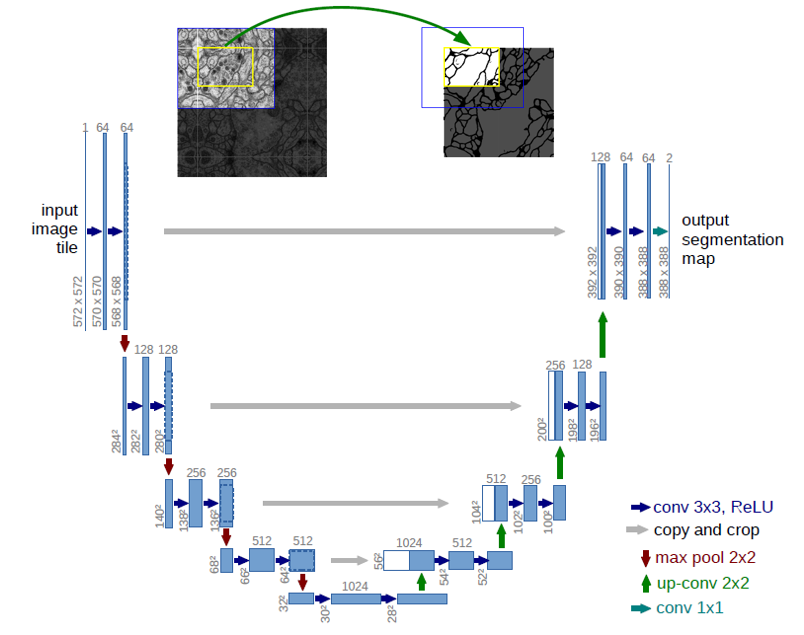
\includegraphics[width=0.9\textwidth]{figures/UNet.png}
        \caption{UNet}
        \label{fig:UNet}
    \end{minipage}
    \begin{minipage}[t]{0.58\textwidth}
        \centering
        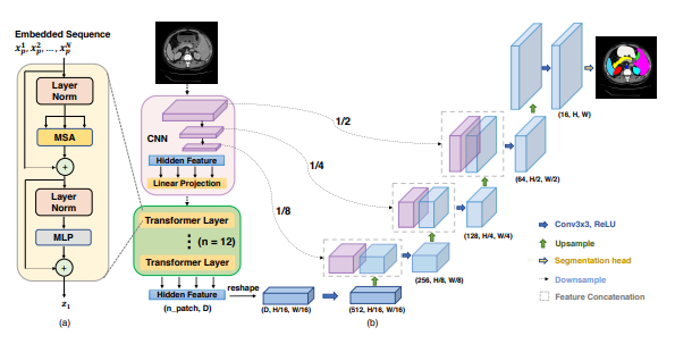
\includegraphics[width=0.8\textwidth]{figures/TransUNet.png}
        \caption{TransUNet}
        \label{fig:TransUNet}
    \end{minipage}
\end{figure}


在医学图像分割任务上一个比较成功的模型是 UNet\cite{UNet}。如图\ref{fig:UNet}所示,UNet 的结构主要分为收缩路径和拓展路径,也有的文献称为编码器和解码器。收缩路径把原始图像下采样到一个比较小的特征图,然后拓展路径再把它上采样回来,模型最终的输出就是对每个像素的分类。

虽然UNet已经在医学图像分割上取得了不错的效果,但是由于卷积操作固有的局部特性,使得它无法对图像中的长程关系进行建模,因此在处理图像中较大的结构时表现出不足。而自然语言处理领域提出的Transformer拥有对全局特征进行建模的强大能力。Alexey Dosovitskiy 等人提出将图像切分成小块并展平为长序列的方法,将 Transformer 引入计算机视觉领域,提出了对图像全局信息具有较强编码能力的 ViT\cite{ViT}。

受到 ViT 启发,Jieneng Chen 等人将 Transformer 应用到 UNet 的编码器中以增强 UNet 提取全局信息的能力,提出了 TransUNet\cite{TransUNet}。TransUNet 的结构如图\ref{fig:TransUNet}所示,在编码器部分,首先用 CNN 处理原图像得到特征图,再对特征图应用 patch embedding,并输入 Transformer 编码得到全局特征;在解码器部分,把特征图跟来自编码器CNN部分的特征图进行拼接,然后经过卷积和激活,再经过上采样一步步放大特征图得到原图像大小的分类结果。得益于 Transformer 对全局信息的强大编码能力和跳跃连接所保留的局部信息,TransUNet 在 Synapse 数据集上达到了当时\footnote{该论文发表于2021年2月8日。}最好的水平。

\section{方法和实验\label{sec:方法和实验}}

\subsection{动机和方法}

\begin{figure}[h]
    \centering
    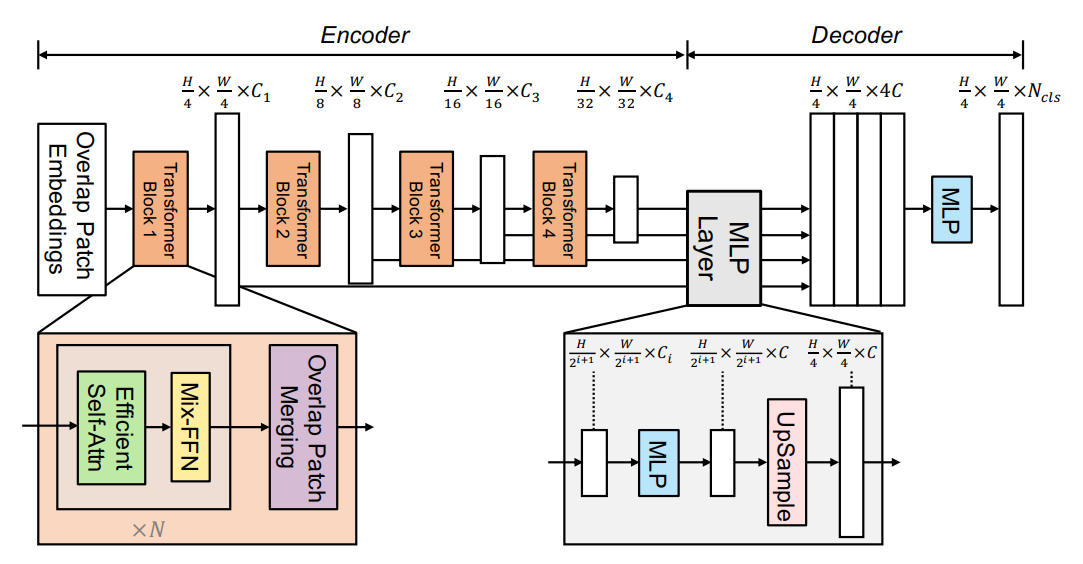
\includegraphics[width=0.8\textwidth]{figures/SegFormer.png}
    \caption{SegFormer}
    \label{fig:SegFormer}
\end{figure}

而在语义分割任务上,由 Enze Xie 等人提出的 SegFormer 模型\cite{SegFormer}(如图 \ref{fig:SegFormer})由层次化的 Transformer 编码器和简单的多层感知机解码器组成,具有结构简单、权重参数少、训练高效和推理速度快等优点。但是,该模型主要用于彩色的生活场景和街道场景图像的语义分割,并未被用于黑白的医学图像分割,论文中也未将 SegFormer 与 TransUNet 进行比较。在本次实验中,我遵循预训练-微调范式,将使用彩色图像预训练的 SegFormer 在 Synapse 和 Lung 数据集上进行微调和测试,探究将彩色场景图象语义分割模型迁移到医学图像分割中的可行性,并将其性能与 TransUNet 在 Synapse 和 Lung 两个医学图像分割数据集上进行对比。

在微调 SegFormer 的过程中,我使用了 AdamW 优化算法和线性学习调度器以加快模型收敛速度和防止过拟合;使用了 early stop 策略,如果连续 6 个 epoch 验证集损失没有下降则停止训练以节省时间;使用了梯度累积技术,在显存不足时使用梯度累积能够防止因 batch size 过小而使参数优化过程不稳定。

\subsection{实验环境}

本次实验在一台 Linux 服务器上完成,显卡型号为 GTX1080Ti,CUDA 版本为 10.1。下面使用 conda 新建 python 虚拟环境,并安装实验所需的 python 软件包:

\begin{lstlisting}[language=bash]
conda create -n TransUNet python=3.7
pip install torch==1.4.0 torchvision==0.5.0 transformers numpy tqdm tensorboard tensorboardX ml-collections medpy SimpleITK scipy nibabel h5py matplotlib datasets
\end{lstlisting}

实验目录结构如下:

\begin{minipage}[c]{0.8\linewidth}
\dirtree{%
    .1 Project.
        .2 \textcolor{cyan}{data}(数据集).
            .3 \textcolor{cyan}{rawSynapse}(原始 Synapse 数据集).
            .3 \textcolor{cyan}{Synapse}(处理后的 Synapse 数据集).
            .3 \textcolor{cyan}{rawLung}(原始 Lung 数据集).
            .3 \textcolor{cyan}{Lung}(处理后的 Lung 数据集).
        .2 \textcolor{cyan}{lists}(数据集列表,指明哪些样例作为训练集,哪些作为测试集).
            .3 \textcolor{cyan}{lists\_Synapse}.
            .3 \textcolor{cyan}{lists\_Lung}.
        .2 \textcolor{cyan}{model}(模型权重参数).
        .2 \textcolor{cyan}{output}(程序输出).
            .3 \textcolor{cyan}{SegFormer}.
                .4 \textcolor{cyan}{Synapse}.
                .4 \textcolor{cyan}{Lung}.
            .3 \textcolor{cyan}{TransUNet}.
                .4 \textcolor{cyan}{Synapse}.
                .4 \textcolor{cyan}{Lung}.
        .2 \textcolor{cyan}{SegFormer}(SegFormer 代码).
        .2 \textcolor{cyan}{TransUNet}(TransUNet 代码).
        .2 \textcolor{green}{process\_synapse.py}(Synapse 数据集预处理脚本).
        .2 \textcolor{green}{process\_lung.py}(Lung 数据集预处理脚本).
        .2 \textcolor{green}{Report.pdf}(实验报告).
}
\end{minipage}

由于数据集和模型权重参数文件较大,我已将其打包上传到\href{https://pan.baidu.com/s/15jhB_8Fxr5q2AzKVAe5yJg?pwd=t2ee}{百度网盘},请下载并解压到 data 和 model 的对应目录下。

\subsection{数据集与预处理}

\subsubsection{Synapse}

TransUNet 原论文使用的数据集 Synapse 是一个人体腹部器官分割的数据集。由于版权问题,TransUNet 的代码仓库中并没有包含模型的训练数据,需要我自行从 \href{https://www.synapse.org/#!Synapse:syn3193805/wiki/}{Synapse 官网} 进行下载。下载得到原始数据集之后,需要对数据集进行以下预处理:

\begin{enumerate}[itemsep=2pt,topsep=0pt,parsep=0pt]
    \item 转换为 numpy 格式;
    \item 重映射标签,因为原数据集有 13 个类别,而原论文只用到了其中 8 个类别,且标签顺序不一致,所以需要将原数据集标签转换为论文所用的标签;
    \item 把图像裁剪到 $[-125, 275]$;
    \item 将每张 3D 图像标准化到 $[0, 1]$;
    \item 训练集:从 3D 图像中提取 2D 切片作为训练样例;测试集: h5 格式的 3D 图像作为测试样例。
\end{enumerate}

以上步骤我通过一个 python 脚本 process\_synapse.py 来完成。

\subsubsection{Lung}

Lung 是一个肺结节医学图像语义分割数据集。该数据集包含 211 位患者在不同时间的肺部 CT 扫描图像,每个 3D 扫描图像和标签已经被处理为 224x224 大小的 2D 切片,格式为 npy。但是,TransUNet 在训练时需要 npz 格式数据,在测试时包含需要 3D 图像的 h5 格式数据,因此需要对该数据集重新进行处理:

\begin{enumerate}[itemsep=2pt,topsep=0pt,parsep=0pt]
    \item 将 211 位患者按照 4:1 的比例随机划分为训练集和测试集;
    \item 对于训练集,将每个 2D 图像和对应标签保存为一个 npz 文件作为训练样例;对于测试集,将某位患者一次扫描的所有切片重新拼接成 3D 数组,保存为 h5 文件作为测试样例。
\end{enumerate}

以上步骤我通过一个 python 脚本 process\_lung.py 来完成。

\subsection{预实验:TransUNet}

为了将从语义分割任务上迁移过来的 SegFormer 模型的性能与 TransUNet 进行对比,我首先复现了 TransUNet 在 Synapse 数据集上的实验结果,并将其应用于 Lung 数据集。

\subsubsection{代码和模型下载}

首先,将 TransUNet 论文的 \href{https://github.com/Beckschen/TransUNet}{代码仓库}克隆到 ./TransUNet 下。然后,下载 TransUNet 所需的 ViT 预训练模型:

\begin{lstlisting}[language=bash]
wget https://storage.googleapis.com/vit_models/imagenet21k/R50+ViT-B_16.npz
mkdir -p ./model/vit_checkpoint/imagenet21k
mv R50+ViT-B_16.npz ./model/vit_checkpoint/imagenet21k/R50-ViT-B_16.npz
\end{lstlisting}

\subsubsection{代码修改}

为了让模型能够在 Lung 数据集上训练,我对代码进行了一些修改,主要有:

\begin{enumerate}[itemsep=2pt,topsep=0pt,parsep=0pt]
    \item 在 train.py 第 64 行的 dataset\_config 中添加 Lung 数据集的信息:
\begin{lstlisting}
'Lung': {
    'root_path': '../data/Lung/train_npz',
    'list_dir': '../lists/lists_Lung',
    'num_classes': 2,
}
\end{lstlisting}
    \item 在 test.py 第 88 行的 dataset\_config 中添加 Lung 数据集的信息:
\begin{lstlisting}
'Lung': {
    'Dataset': Synapse_dataset,
    'volume_path': '../data/Lung/test_vol_h5',
    'list_dir': '../lists/lists_Lung',
    'num_classes': 2,
    'z_spacing': 1,
}
\end{lstlisting}
    \item 由于训练集路径等信息已经在 dataset\_config 中给出,因此从 train.py 中删去冗余的命令行参数 root\_path、list\_dir 和 num\_classes;
    \item 同理从 test.py 中删去冗余的命令行参数 volume\_path、list\_dir 和 num\_classes。
\end{enumerate}

\subsubsection{训练与测试}

使用如下命令可以分别在 Synapse 和 Lung 数据集上训练 TransUNet:

\begin{lstlisting}[language=bash]
cd TransUNet
python train.py --dataset Synapse --vit_name R50-ViT-B_16 --batch_size 22 \
    > ../output/TransUNet/Synapse/train.log
python train.py --dataset Lung --vit_name R50-ViT-B_16 --batch_size 24 \
    > ../output/TransUNet/Lung/train.log
\end{lstlisting}

训练日志会保存到 ./output/TransUNet 下,模型权重参数会保存到 ./model/TransUNet 下。

使用如下命令可以加载训练时保存的模型参数并分别在 Synapse 和 Lung 数据集上测试 TransUNet:

\begin{lstlisting}[language=bash]
cd TransUNet
python test.py --dataset Synapse --vit_name R50-ViT-B_16 --batch_size 22 \
    --max_epochs 150 > ../output/TransUNet/Synapse/test.log
python test.py --dataset Lung --vit_name R50-ViT-B_16 --batch_size 24 \
    --max_epochs 150 > ../result/TransUNet/Lung/test.log
\end{lstlisting}

测试结果将保存到 ./output/TransUNet 下。

\subsection{主实验:SegFormer}

论文作者已将不同大小的 SegFormer 预训练模型开源在了 \href{https://huggingface.co/}{Hugging Face} 社区,我们需要加载该预训练模型并在两个数据集上进行微调。我在微调过程中使用了 AdamW 优化算法、线性学习率衰减、early stop 策略和梯度累积等技术。下面对程序进行详细介绍:

./SegFormer 目录下包含 4 个 python 程序文件,其中,位于 ./SegFormer/utils 下的 datasets.py 和 metrics.py 两个模块分别用于加载数据集和计算评价指标,相关代码由 TransUNet 源码修改得到,不多赘述。下面,主要介绍 train.py 中的训练和测试函数,还有启动脚本 main.py。

\subsubsection{启动脚本}

启动脚本 main.py 主要功能如下:

\begin{enumerate}[itemsep=2pt,topsep=0pt,parsep=0pt]
    \item 定义和解析命令行参数;
    \item 使用 transformers 模块加载 SegFormer 预训练模型;
    \item 命令行参数 test 表示是否只进行测试,若它被设置为 False,则加载训练集并调用 train() 微调模型;
    \item 加载训练时保存的最好的模型参数;
    \item 调用 test() 进行测试。
\end{enumerate}

\subsubsection{训练函数}

位于 trainer.py 中的训练函数 train() 的主要功能是微调 SegFormer 模型,函数的流程如下:

\begin{enumerate}[itemsep=2pt,topsep=0pt,parsep=0pt]
    \item 定义 logger,以便将训练日志同时输出到终端和文件;
    \item 将训练集按照 4:1 的比例随即切分为训练集和验证集;
    \item 定义数据加载器、优化器和学习率调度器,使用 AdamW 优化算法和线性衰减学习率调度;
    \item 对于每个 epoch:
    \begin{enumerate}[itemsep=2pt,topsep=0pt,parsep=0pt]
        \item 对于训练集中每个 batch 的数据:
        \begin{enumerate}[itemsep=2pt,topsep=0pt,parsep=0pt]
            \item 将数据输入模型得到输出并计算损失;
            \item 反向传播计算梯度;
            \item 当累积了指定步数时进行一次参数更新并清空梯度和调整学习率;
        \end{enumerate}
        \item 对于验证集中每个 batch 的数据,同样使用 mini-batch 方法得到计算损失,但是不用进行反向传播,最终得到当前模型在整个验证集的平均损失;
        \item 若当前模型在验证集上的损失小于之前的最小损失,则保存当前模型参数,当模型连续若干个 epoch 验证集损失没有下降时,停止训练;
    \end{enumerate}
    \item 绘制训练过程训练集和验证集平均损失变化曲线。
\end{enumerate}

\subsubsection{测试函数}

位于 trainer.py 中的训练函数 test() 的主要功能是使用训练好的 SegFormer 模型在测试集上推理并计算评价指标,流程如下:

\begin{enumerate}[itemsep=2pt,topsep=0pt,parsep=0pt]
    \item 定义 logger,以便将测试日志同时输出到终端和文件;
    \item 对于每个 3D 的测试样例:
    \begin{enumerate}[itemsep=2pt,topsep=0pt,parsep=0pt]
        \item 在第一个维度上进行切片,将每个切片输入模型得到输出,然后将输出通过双线性插值上采样到原图像大小,得到预测结果,最后把每个切片的预测结果拼起来得到整个样例的预测结果;
        \item 计算评价指标;
    \end{enumerate}
    \item 将每个样例的评价指标取平均得到整个测试集上的评价指标。
\end{enumerate}

\subsubsection{训练与测试}

使用如下命令可以分别在 Synapse 和 Lung 数据集上微调 SegFormer 模型:

\begin{lstlisting}[language=bash]
cd SegFormer
python main.py --pretrained_model nvidia/mit-b0 --dataset Synapse \
    --batch_size 16 --accumulate_steps 1
python main.py --pretrained_model nvidia/mit-b0 --dataset Lung  \
    --img_size 224 --batch_size 16 --accumulate_steps 1
\end{lstlisting}

其中,pretrained\_model 用于选择预训练模型,一共有 6 种大小的预训练模型可供选择,对于较大的模型可能需要调整 batch\_size 和 accumulate\_steps 参数以免显存不够。

程序在训练结束时会自动进行测试并记录结果,但如果您想单独运行测试,可以使用如下命令:

\begin{lstlisting}[language=bash]
cd SegFormer
python main.py --pretrained_model nvidia/mit-b0 --dataset Synapse --test True
python main.py --pretrained_model nvidia/mit-b0 --dataset Lung  \
    --img_size 224 --test True
\end{lstlisting}


\section{实验结果与分析\label{sec:实验结果与分析}}

我将 TransUNet 原论文报告的结果、我复现的结果以及 6 种大小的 SegFormer 的结果汇总在表\ref{tab:测试集结果}中。接下来我从多个方面对结果进行细致的对比分析。

\begin{table}[ht!]
    \centering
    \caption{测试集结果}
    \label{tab:测试集结果}
    \begin{tabular}{c|c|c|c|c}
        \multirow{2}{*}{\textbf{模型}} & \multicolumn{2}{c|}{\textbf{Synapse}} & \multicolumn{2}{c}{\textbf{Lung}}\\
            & DSC$\uparrow$ & HD$\downarrow$ & DSC$\uparrow$ & HD$\downarrow$\\
        \hline
        TransUNet(原论文) & 77.48 & 31.69 & / & / \\
        TransUNet(复现) & 77.93 & 30.69 & 79.55 & 1.88 \\
        \hline
        SegFormer-B0 & 74.88 & 33.80 & 76.00 & 4.46 \\
        SegFormer-B1 & 77.34 & 32.08 & 78.33 & 5.44 \\
        SegFormer-B2 & 79.60 & 32.30 & 80.48 & 3.72 \\
        SegFormer-B3 & 79.10 & 36.20 & 78.76 & 4.21 \\
        SegFormer-B4 & 81.30 & 31.40 & 78.31 & 5.97 \\
        SegFormer-B5 & 81.64 & 28.29 & 78.83 & 5.19
    \end{tabular}
\end{table}

\subsection{TransUNet 复现效果}

\begin{table}[ht!]
    \centering
    \caption{TransUNet 复现效果(DSC)}
    \label{tab:TransUNet复现效果}
    \begin{tabular}{c|c|c|c|c|c|c|c|c}
        \textbf\small{TransUNet} & \textbf\small{Aorta} & \textbf\small{Gallbladder} & \textbf\small{Kidney(L)} & \textbf\small{Kidney(R)} & \textbf\small{Liver} & \textbf\small{Pancreas} & \textbf\small{Spleen} & \textbf\small{Stomach}\\
        \hline
        原论文 & 87.23 & 63.13 & 81.87 & 77.02 & 94.08 & 55.86 & 85.08 & 75.62 \\
        复现 & 87.25 & 64.61 & 82.53 & 78.25 & 94.18 & 58.43 & 83.59 & 74.58
    \end{tabular}
\end{table}

如表\ref{tab:测试集结果}和表\ref{tab:TransUNet复现效果}所示,我复现的 TransUNet 在 Synapse 测试集上的各器官的 DSC 与原论文报告的结果十分相近,而在整个测试集上的平均 DSC 和 HD 略好于原论文结果,说明复现成功。

\subsection{SegFormer 模型大小对结果的影响}

\begin{figure}[h]
    \centering
    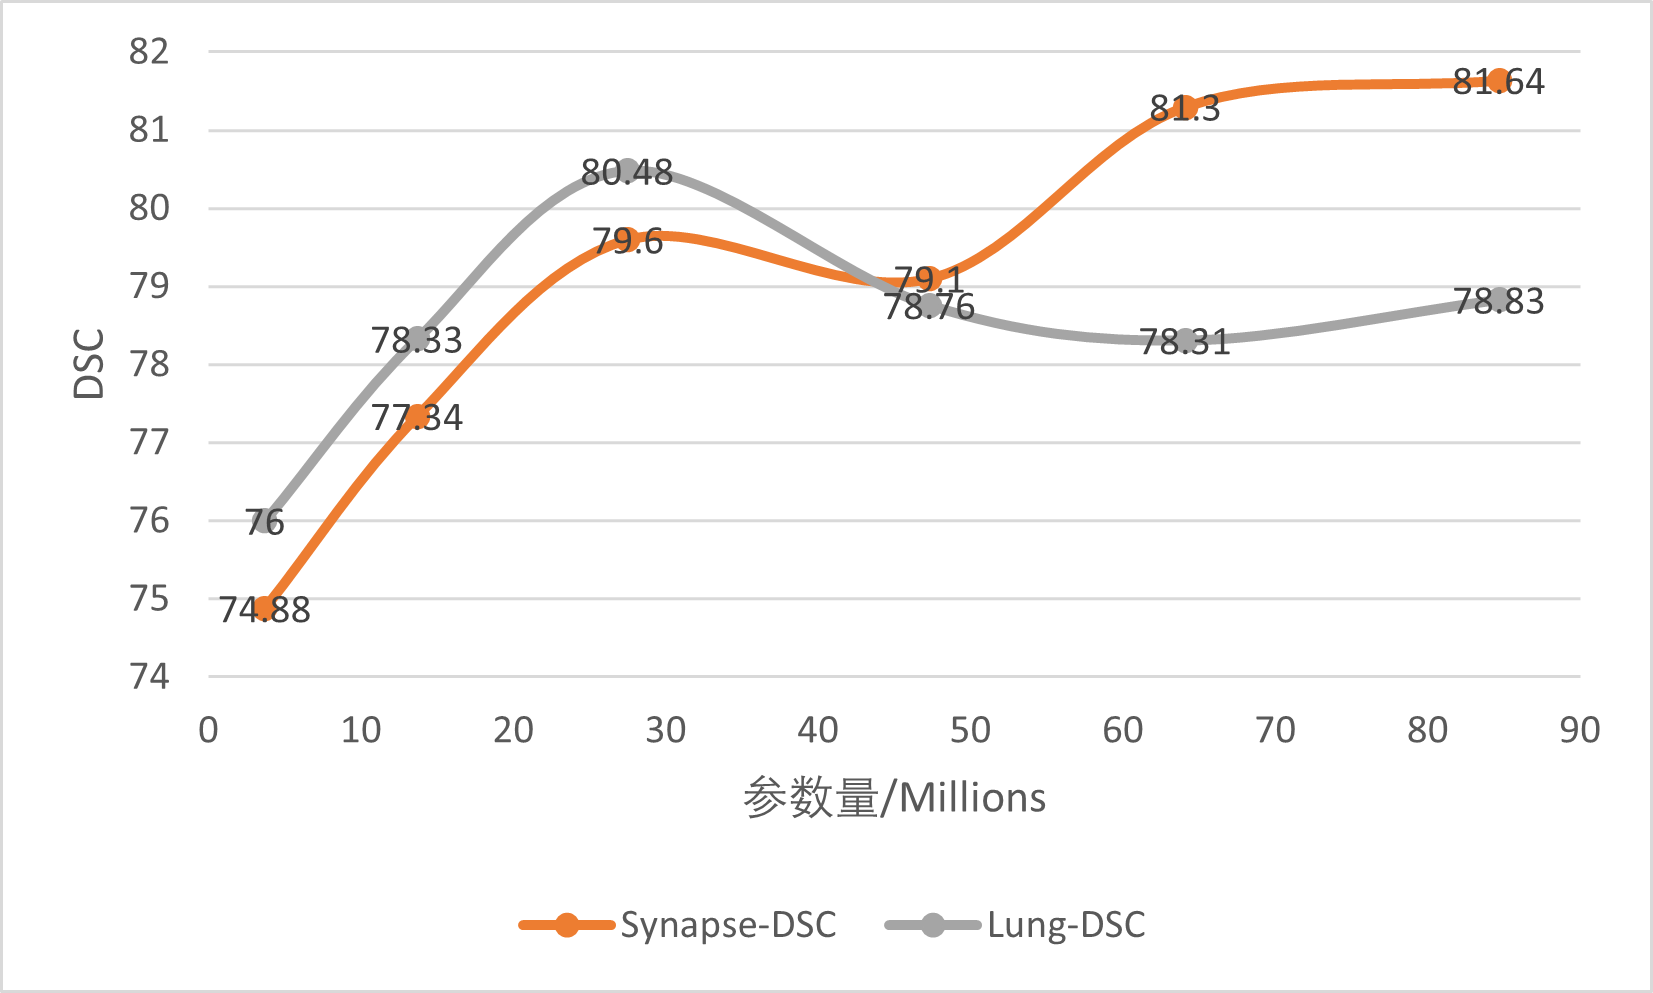
\includegraphics[width=0.8\textwidth]{figures/SegFormer模型大小对结果的影响.png}
    \caption{SegFormer 模型大小对结果的影响}
    \label{fig:SegFormer模型大小对结果的影响}
\end{figure}

从 SegFormer-B0 到 SegFormer-B5,模型参数量依次递增,它们在两个数据集上的表现如表\ref{tab:测试集结果} 和图 \ref{fig:SegFormer模型大小对结果的影响} 所示。

如图\ref{fig:SegFormer模型大小对结果的影响},不同大小的 SegFormer 模型在 Synapse 数据集上的表现基本符合原论文\cite{SegFormer}的结论,即模型越大效果越好,但是存在边际效应:刚开始时,增加模型参数量能够增强模型表达能力,使性能快速提升;但是当参数量较大时,继续增加参数量,模型性能提升幅度减小。但是对于 Lung 数据集,当模型参数大于 30M 时,性能反而下降,这可能是由于 Lung 只有 2 个类别,比较简单,因此大模型更容易对训练集过拟合,导致在测试集上分数下降。

\subsection{TransUNet 与 SegFormer 比较}

\subsubsection{DSC}

如表\ref{tab:测试集结果}所示,6 种不同大小的 SegFormer 模型中,有 4 个在 Synapse 数据集上的 DSC 分数超过了复现的 TransUNet 模型,最多超过了 3.71;有 1 个在 Lung 数据集上的 DSC 分数超过了复现的 TransUNet 模型,超过了 0.93。这说明,SegFormer 模型应用在医学图像语义分割上\textbf{能够}得到不错的效果。

\subsubsection{模型参数量}

TransUNet 模型参数量为 93.192 M\footnote{数据使用 thop 工具计算得到。\label{foot:thop}},浮点运算数(FLOPs)为 128.677 G\textsuperscript{\ref{foot:thop}};而不同 SegFormer 模型参数量在 3.7 $\sim$ 84.7 M\footnote{数据来自原论文\cite{SegFormer}。\label{foot:数据来自原论文}} 之间,仅需参数量为 27.5 M\textsuperscript{\ref{foot:数据来自原论文}}、浮点运算数为 64.24 G\textsuperscript{\ref{foot:数据来自原论文}} 的 SegFormer-B2 在两个数据集上的 DSC 分数都超过了 TransUNet 模型。由参数量和浮点运算数的减少带来的推理速度的提升为医学图像的实时语义分割提供了可能。

\section{结论\label{sec:结论}}

在本次实验中,我成功复现了 TransUNet 在 Synapse 上的结果,并将其用于 Lung 数据集。我还将原本用于彩色场景图像语义分割的 SegFormer 模型迁移到医学图像语义分割任务上,在上述两个数据集上得到了超过 TransUNet 的结果,证明了利用预训练-微调范式将其他领域语义分割模型迁移到医学图像语义分割上的有效性。我还对比分析了 SegFormer 和 TransUNet 的参数量,说明了将 SegFormer 应用到医学图像语义分割能够带来速度上的提升,为实时应用提供了可能。

\section{讨论与改进方向\label{sec:讨论与改进方向}}

虽然 SegFormer 模型应用在医学图像语义分割上能够得到不错的效果,但是它存在如下劣势:

\begin{enumerate}[itemsep=2pt,topsep=0pt,parsep=0pt]
    \item 在 3 通道的彩色图像上预训练,而医学图像多为单通道的黑白图像,所提供的信息量更少;
    \item 在日常生活场景或街道场景上预训练,对物品、车辆和人物等进行语义分割与对病理学结构进行语义分割差距较大,预训练过程中很难学到病理学结构的语义知识;
    \item 大模型在有几百个类别的预训练任务上能够表现很好,但病理学语义分割类别较少,有的甚至只有两类,容易造成过拟合;
    \item 如图\ref{fig:SegFormer}所示,SegFormer 模型最终的输出只有原图像的 1/4 大小,需要通过双线性插值的方法上采样到原大小,而在 TransUNet 论文\cite{TransUNet}中已经用实验表明,双线性插值上采样器效果劣于级联的转置卷积上采样器;双线性插值上采样的方法可能不能满足医学图像分割的精度要求。
\end{enumerate}

针对以上劣势,我提出以下可能的对 SegFormer 的改进方向:

\begin{enumerate}[itemsep=2pt,topsep=0pt,parsep=0pt]
    \item \textbf{在灰度图像上预训练}:虽然由于病理学语义分割数据的标注较为昂贵,无法使用大量病理学语义分割数据进行预训练,但是我可以将大量的其他语义分割数据集处理为单通道的灰度图像进行预训练,以提高模型从灰度图像中提取信息的能力;
    \item \textbf{使用自监督方法在医学图像上对编码器进行预训练}:对比学习等自监督方法能够在无标注数据的情况下对编码器进行预训练,从而提高编码器从医学图像中提取信息的能力,而这种方法尤其适用于 SegFormer,因为 SegFormer 的权重参数大部分集中与编码器,解码器仅为简单的多层感知机;
    \item \textbf{提高模型输出的分辨率}:医学图像分割对分割精度有更高要求,虽然提高模型输出分辨率会增加模型参数,但这种参数的增加可能是值得的;
    \item \textbf{使用级联的转置卷积上采样器}:使用效果更好的级联的转置卷积上采样器取代 SegFormer 中的多层感知机和双线性插值上采样器,或许能够提升模型输出的精度。
\end{enumerate}

限于时间原因,我未能在本次实验中对以上改进方案进行尝试,但我希望在未来能够对这些改进方案进行探究。


\begin{thebibliography}{99}
\bibitem{UNet}Olaf Ronneberger, Philipp Fischer, Thomas Brox: U-net: Convolutional networks for biomedical image segmentation. In: International Conference on Medical image computingand computer-assisted intervention. pp. 234-241. Springer (2015)
\bibitem{ViT}Alexey Dosovitskiy, Lucas Beyer, Alexander Kolesnikov, Dirk Weissenborn, Xiaohua Zhai, et al.: An image is worth 16x16 words: Transformers for image recognition at scale. In: ICLR (2021)
\bibitem{TransUNet}Jieneng Chen, Yongyi Lu, Qihang Yu, Xiangde Luo, Ehsan Adeli, Yan Wang, Le Lu, Alan L. Yuille, and Yuyin Zhou: TransUNet: Transformers Make Strong
Encoders for Medical Image Segmentation. arXiv:2102.04306 (2021).
\bibitem{CETR}Sixiao Zheng, Jiachen Lu, Hengshuang Zhao, Xiatian Zhu, Zekun Luo, Yabiao Wang, Yanwei Fu, Jianfeng Feng, Tao Xiang, Philip HS Torr, et al. Rethinking semantic segmentation from a sequence-to-sequence perspective with transformers. CVPR, 2021.
\bibitem{SegFormer}Enze Xie, Wenhai Wang, Zhiding Yu, Anima Anandkumar3,, Jose M. Alvarez, Ping Luo: SegFormer: Simple and Efficient Design for Semantic Segmentation with Transformers. arXiv:2105.15203 (2021).
\end{thebibliography}

\end{document}